\documentclass[11pt, oneside]{article}
\usepackage{geometry}
\geometry{letterpaper}
\usepackage{amsmath}
\usepackage{graphicx}
\usepackage{amssymb}
\graphicspath{{Visuels/}}
\usepackage[francais]{babel}
\usepackage[utf8]{inputenc}



\title{\begin{center} Algorithme de Préférence : Pass Culture \end{center}}

\author{Paul Garnier \\ François Remili \\ Arthur Verrez}


\begin{document}


\maketitle


\pagestyle{empty}

\maketitle





\pagestyle{plain}

\section{Concepts Principaux}

On cherche à proposer aux utilisateurs les offres qui leur correspondent. Dans un deuxième temps, on va chercher à étendre ces offres pour agrandir le potentiel culturel de chacun des utilisateurs. Pour ce faire, on va d'abord considérer des matrices "caractéristiques" des utilisateurs et des offres. \\

D'un point de vue théorique, notons :

\begin{center}

 $\;\;\;\;\;\;\;\;\mathcal{U} = \{U_i \; ; \; i \in \mathbb{N} \}$ l'ensemble des utilisateurs \\
$\mathcal{O} = \{O_i \; ; \; i \in \mathbb{N} \}$ l'ensemble des offres \\

\end{center}

ainsi que $N_1$ le nombre des tags principaux ("Théâtre", "Peinture", "Opéra", ...) et $N_2$ le nombre de tags secondaires ("Français", "Italien", "Familial", ...). \\

À chaque $O_i$ et $U_i$ on associe donc, comme dit plus haut, une matrice des caractéristiques. D'un point de vue informatique, on les appellera par $U_i$.préférence et $O_i$.préférence. Ici, mathématiquement, on les notera $\mathcal{M} (U_i)$ et $\mathcal{M} (O_i)$. Ces matrices seront de tailles $N_2 \times N_1$.

\begin{center}
\[
\mathcal{M} (O_i) =
\begin{pmatrix}
a_{1,1} & \cdots & a_{1,N_1} \\
\vdots & & \vdots \\
a_{N_2,1} & \cdots & a_{N_2,N_1}
\end{pmatrix}
\]
où :
\[
 \left \{
   \begin{array}{r c l}
      \forall i,j \; \; & 0 \leq a_{i,j} \leq 1 \\
      \displaystyle \sum_{i,j} a_{i,j}^{2} &=& 1 \\
   \end{array}
   \right .
\]
\end{center}

La somme des carrés des coefficients de la matrice égale à $1$ signifie que la matrice est normalisée pour la norme euclidienne sur $\mathcal{M}_{N2,N1} $ : on travaille donc avec des éléments de la sphère unité de ce même espace, dont tous les coefficients sont positifs. Cette norme est issu du produit scalaire  que l'on retrouvera pour notre fonction attraction (représentant littéralement l'attraction entre un utilisateur et une offre). \\

En effet, on définit donc une fonction attraction $\phi$ :

\begin{center}
\[
\begin{array}{l|rcl}
\phi : & \big( \mathcal{M}_{N_2,N_1} \big)^{2} & \longrightarrow & [0,1] \\
    & (A,B) & \longmapsto & \displaystyle \sum _{k,l} a_{k,l}b_{k,l} \end{array}
\]

\end{center}

Par la normalisation des matrices préférences ainsi que par la définition de $\phi$ (c'est un produit scalaire), on peut utiliser l'inégalité de Cauchy-Schwarz pour s'assurer que $\forall i,j$, on a $\phi (\mathcal{M} (U_i)$,$\mathcal{M} (O_j)) \in [0,1]$. Finalement, plus cette fonction est proche de $1$, plus l'événement est censé plaire à notre utilisateur : le produit scalaire est maximal et égal à $1$ si, et seulement si, les deux matrices de préférences sont égales. \\ On renverra donc en priorité l'offre $O_j$ qui maximise cette fonction attraction pour notre utilisateur.  \\

De la même façon, on va introduire une fonction "ressemblance" $\Theta$ entre deux utilisateurs et une autre pour deux événements $\theta$ :

\begin{center}
\[
\begin{array}{l|rcl}
\Theta : &  \mathcal{U}^{2} & \longrightarrow & [0,1] \\
    & (U_i,U_j) & \longmapsto & \Theta (U_i,U_j) \end{array}
\begin{array}{l|rcl}
\theta : & \mathcal{O}^{2} & \longrightarrow & [0,1] \\
    & (O_i,O_j) & \longmapsto & \theta (O_i,O_j) \end{array}
\]
\end{center}

On va aussi définir une fonction $\mathcal{V}$ représentant le potentiel d'un utilisateur $U_i$ pour évaluer un événement $O_i$ :
\begin{center}
\[
\begin{array}{l|rcl}
\mathcal{V} : & \mathcal{U} \times \mathcal{O} & \longrightarrow & [0,1] \\
    & (U_i,O_j) & \longmapsto & \mathcal{V} (U_i,O_j) \end{array}
\]

\end{center}

On va ainsi construire ces différentes fonctions pour pouvoir constamment modifier les matrices  $\mathcal{M} (U_i)$ et $\mathcal{M} (O_i)$. Il faudra d'abord prendre en compte l'utilisateur précisément : ce qu'il choisit, ce qu'il ne choisit pas et comment cela modifie sur les matrices. Ensuite, il faudra prendre en compte ce que les utilisateurs qui lui ressemblent font. Finalement, on prendra aussi en compte ce que l'utilisateur choisit, non pas pour modifier les matrices mais pour directement changer les offres recommandées.

\section{Le cas de l'utilisateur seul}

Considérons d'abord ce qui ce passe à partir du moment où des offres sont proposées à l'utilisateur. On considère qu'une offre "vue" mais non "swipe up" peut toujours changer d'état si l'utilisateur revient dessus. Il existe aussi des offres tout simplement "non vue". Ainsi, si l'on note $\mathcal{OP}$ pour offres proposées l'ensemble de ces offres, on peut le partitionner comme suit :

\begin{center}

$\mathcal{OP} = \mathcal{L} \cup \mathcal{UL} \cup \mathcal{US}$

\end{center}

où $\mathcal{L}$ sont les offres swipe up, $\mathcal{UL}$ les offres non swipe up et $\mathcal{US}$ les offres non vues. On notera $S = \#\mathcal{L} + \#\mathcal{UL}$. On va s'intéresser précisément à chacun de ces trois ensembles. \\

\textbf{Le cas de $\mathcal{L}$} : \\

On note ici l'utilisateur $U_{i_0} \in \mathcal{U}$ et l'événement $O_{j_0} \in \mathcal{O}$. On sait déjà qu'il est intéressé par l'événement en question. On va donc modifier leurs matrices respectives. Dans le cas d'un événement "swipe up", on va modifier les matrices sur tous leurs coefficients (ce ne sera pas le cas pour l'ensemble $\mathcal{UL}$. Il faut prendre en compte différents facteurs : le nombre d'utilisateur $\#\mathcal{U}$, sa faculté à influencer l'événement $\mathcal{V}$ et finalement deux facteurs multiplicatifs $\alpha$ et $\beta$ pour pouvoir jouer sur le changement des matrices. \\

Pour les matrices $\mathcal{M} (U_i)$ (resp. $\mathcal{M} (O_i)$), on considère un coefficient arbitraire $a_{p,q}$ (resp. $b_{p,q}$), et on va réaliser l'opération suivante :
\begin{center}
\[
 \big( a_{p,q} \times \frac{S}{S+1} + b_{p,q}\times \frac{1}{S+1} \big) 
\]
\end{center}
et on remplace $a_{p,q}$ par ce que l'on vient de calculer.

De la même façon, on remplace $b_{p,q}$ par :
\begin{center}
\[
 \big( b_{p,q} \times \frac{S}{S+1} + a_{p,q}\times \frac{1}{S+1}) \big( \times \frac{\mathcal{V}(U_{i_0},O_{j_{0}})}{\#\mathcal{U}})
\]
\end{center}

On prendrait ensuite soin de renormaliser les deux matrices de préférences en divisant chacun de leur coefficients par leur "norme intermédiaire". Plus géométriquement, les opérations que l'on décrit ici reviennent à projeter un barycentre avec des poids bien choisis entre deux matrices de préférences sur la sphère unité de $ \mathcal{M}_{N2,N1} $. \\

talk autour des coefficients : (todo) \\

\textbf{Le cas de $\mathcal{UL}$} : \\

Il semblerait qu'ici, on puisse se contenter de réaliser les mêmes calculs mais avec les coefficients conjugués. On introduit tout de même deux nouveaux coefficients $\tilde{\alpha}$ et $\tilde{\beta}$. De plus, on n'utilise pas pour le moment, dans ce cas précis, la fonction $\mathcal{V}$. On va donc ajouter à $a_{p,q}$ et à $b_{p,q}$:
\begin{center}
\[
 \big( a_{p,q} \times \frac{S}{S+1} + (1 - b_{p,q})\times \frac{1}{S+1} \big) \times\tilde{\alpha}
\]
\end{center}
et :
\begin{center}
\[
 \big( b_{p,q} \times \frac{S}{S+1} + (1 - a_{p,q})\times \frac{1}{S+1}) \big( \times \frac{\mathcal{\tilde{\beta}}}{\#\mathcal{U}}
\]
\end{center}

\textbf{Le cas de $\mathcal{US}$} : \\

On considère ici qu'un événement non vu est voué à l'être. On ne modifie donc rien pour les événements proposés mais non vus. Il n'y a donc pas de changement. C'est cependant un ensemble à prendre en compte d'un point de vue algorithmique dans tout nos programmes.



\section{Interactions entre les différents utilisateurs}

On se donne un entier $k \in \mathbb{N}$, et on considère l'ensemble :
\begin{center} $\mathcal{N} _k (U_i) = \{ U_j \; \text{telle que} \; \Theta (U_i,U_j) \; \text{soit l'une des} \; k\; \text{plus grandes valeurs} \} $ \end{center}
On ne va considérer que ces $k$ utilisateurs pour influencer la matrice de notre utilisateur ainsi que celles des événements dans $\mathcal{L}$. Il faut tout de même avoir défini avant cela la fonction $\Theta$, considérons pour le moment que c'est la même fonction attraction $\phi$, comme défini au début du document. Plus que la simple fonction $\phi$ d'attraction, on peut calculer une seconde fonction d'attraction, grâce aux autres utilisateurs. Cette fonction se base plus ou moins sur une interprétation des Relations de Chasles. Notons $\psi$ la quantité suivante :
\begin{center}
\[
\psi (U_i,O_j) = \frac{\displaystyle \sum _{p \in \mathcal{N} _k (U_i)} \Theta (U_i,p) \times \phi (p,O_j)}{\displaystyle \sum _{p \in \mathcal{N} _k (U_i)} \Theta (U_i,p)}
\]
\end{center}

C'est une nouvelle fonction d'attraction qui prend ici en compte les autres utilisateurs. On va l'utiliser pour modifier les matrices de préférences d'un utilisateur. On note $\Delta$ la fonction suivante :
\begin{center}
\[
\begin{array}{l|rcl}
\Delta : & \mathcal{U} \times \mathcal{O} & \longrightarrow & [0,1] \\
    & (U_i,O_j) & \longmapsto & \frac{1}{2} \left| \psi(U_i,O_j) - \phi(U_i,O_j)   \right| \end{array}
\]

\end{center}

On va utiliser cette fonction maintenant, et on l'utilisera aussi ensuite pour proposer directement des nouveaux événements. Pour la modification des matrices, on va chercher à comprendre pourquoi il peut y avoir une telle différence entre $\phi$ et $\psi$. \\
 Si $\psi(U_i,O_j) \leq \phi(U_i,O_j)$, on ne s'y intéresse pas. En revanche, si l'on a $\phi(U_i,O_j) \leq \psi(U_i,O_j)$, il faut chercher à comprend quels coefficients des matrices en sont la cause. Considérons, de façon arbitraire pour le moment, que l'on ne va modifier que $5$ coefficients. On note tout de même $n$ cet entier. \\
On note $\mathcal{I} (U_i,O_j$ l'ensemble à $2n$ élément qui se constitue des couples $(p,q)$ lié aux produits $a_{k,l}b_{k,l} $ les plus importants. \\
On considère maintenant $\mathcal{J}$ l'intersection de ces ensembles :
\begin{center}
\[
\mathcal{J} = \bigcap _{p \in \mathcal{N} _k (U_i) } \mathcal{I} (p,O_j)
\]

\end{center}

Finalement, on va enfin modifier les bon coefficients $\{a_{p,q} \; ; \; (p,q) \in \mathcal{J} \} $ en les remplaçant par :
\begin{center}
\[
 \left \{
   \begin{array}{r c l}
       a_{p,q} + \frac{\Delta (U_i,O_j)}{2} \;  &\text{si}& \; a_{p,q} + \Delta (U_i,O_j) \leq 1  \\
       \frac{ a_{p,q} + 1}{2} &\text{sinon}& \\
   \end{array}
   \right .
\]
\end{center}

On va maintenant voir comment les autres utilisateurs peuvent directement influencer les offres proposées. Il nous suffit de remplacer la fonction d'attraction $\phi$ par $\psi$. On récupère ainsi les offres proposées par $\psi$ et pas par $\phi$, et on les injecte avec une proportion de $z \%$.

\section{Dernière façon de proposer des événements}

Toujours dans l'optique d'étendre le champ culturel de l'utilisateur, cherchons une autre façon de lui proposer des événements. Pour ce faire, on va s'intéresser aux tags secondaires. On reste encore sur un utilisateur $U_{i_0}$ fixé. On note encore $\mathcal{M} (U_{i_0})$ sa matrice préférence. On note $\mathcal{T}^2$ de cardinal $N_2$ l'ensemble des tags secondaires. On note $\mathcal{T}^2_{U_i}$ l'ensemble ordonné des tags secondaires pour l'utilisateur $U_i$ par l'ordre naturel sur la somme des coefficients de sa ligne dans la matrice $\mathcal{M} (U_{i})$ par exemple. On utilise des notations symétrique pour les tags principaux avec $\mathcal{T}^1$. \\
On note finalement $(p_0,q_0)$ le couple tel que $p_0$ corresponde au premier élément de $\mathcal{T}^2_{U_i}$ et $q_0$ au dernier élément de $\mathcal{T}^1_{U_i}$. On récupère enfin les offres de $\mathcal{O}$ qui possède le coefficient $(p_0,q_0)$ les plus élevés. On note $\mathcal{O}_{p_0,q_0}^y$ cet ensemble, où $y = \# \mathcal{O}_{p_0,q_0}^y$. \\

Il ne nous reste plus qu'à appliquer notre fonction d'attraction $\phi$ à cet ensemble, et à proposer ces offres à l'utilisateur avec une proportion $\tilde{z} \%$.

\section{Autour de la Diversification}

L'idée ici est de discuter des différentes façons de mesurer la diversification d'un utilisateur. Par diversification, on entend la capacité qu'a l'utilisateur de s'éloigner de ce qu'il aime pour découvrir de nouvelles choses. À cette notion est liée deux problèmes : d'abord, comment mesurer la diversification. Ensuite, comme faire pour l'augmenter? On élabore ici différente manière de mesurer la diversification, puis comment la faire évoluer. 

\subsection{Méthode 1} 

On considère encore une fois notre matrice utilisateur $\mathcal{M} (U_i)$ de coefficients $a_{i,j}$. On considère la fonction suivante : 

\begin{center}
\[
\begin{array}{l|rcl}
\mathcal{D} : &  \mathcal{M}_{N_2,N_1} & \longrightarrow & [0,1] \\
    & \mathcal{M} (U_i) & \longmapsto & \frac{1}{\sqrt{N_2 N_1}} \displaystyle \sum _{k,l} a_{k,l}
    \end{array}
\]

\end{center}

Concrétement, cette fonction représente le produit scalaire entre notre matrice et la matrice constituée que de $1$ normalisée. On cherche donc, pour mesurer la diversification, à étudier l'écart entre l'utilisateur et un utilisateur référence qui aime tout de manière égale. \\

\begin{figure}[h]
   \caption{Méthode 1 avec des vecteurs non normalisés}
   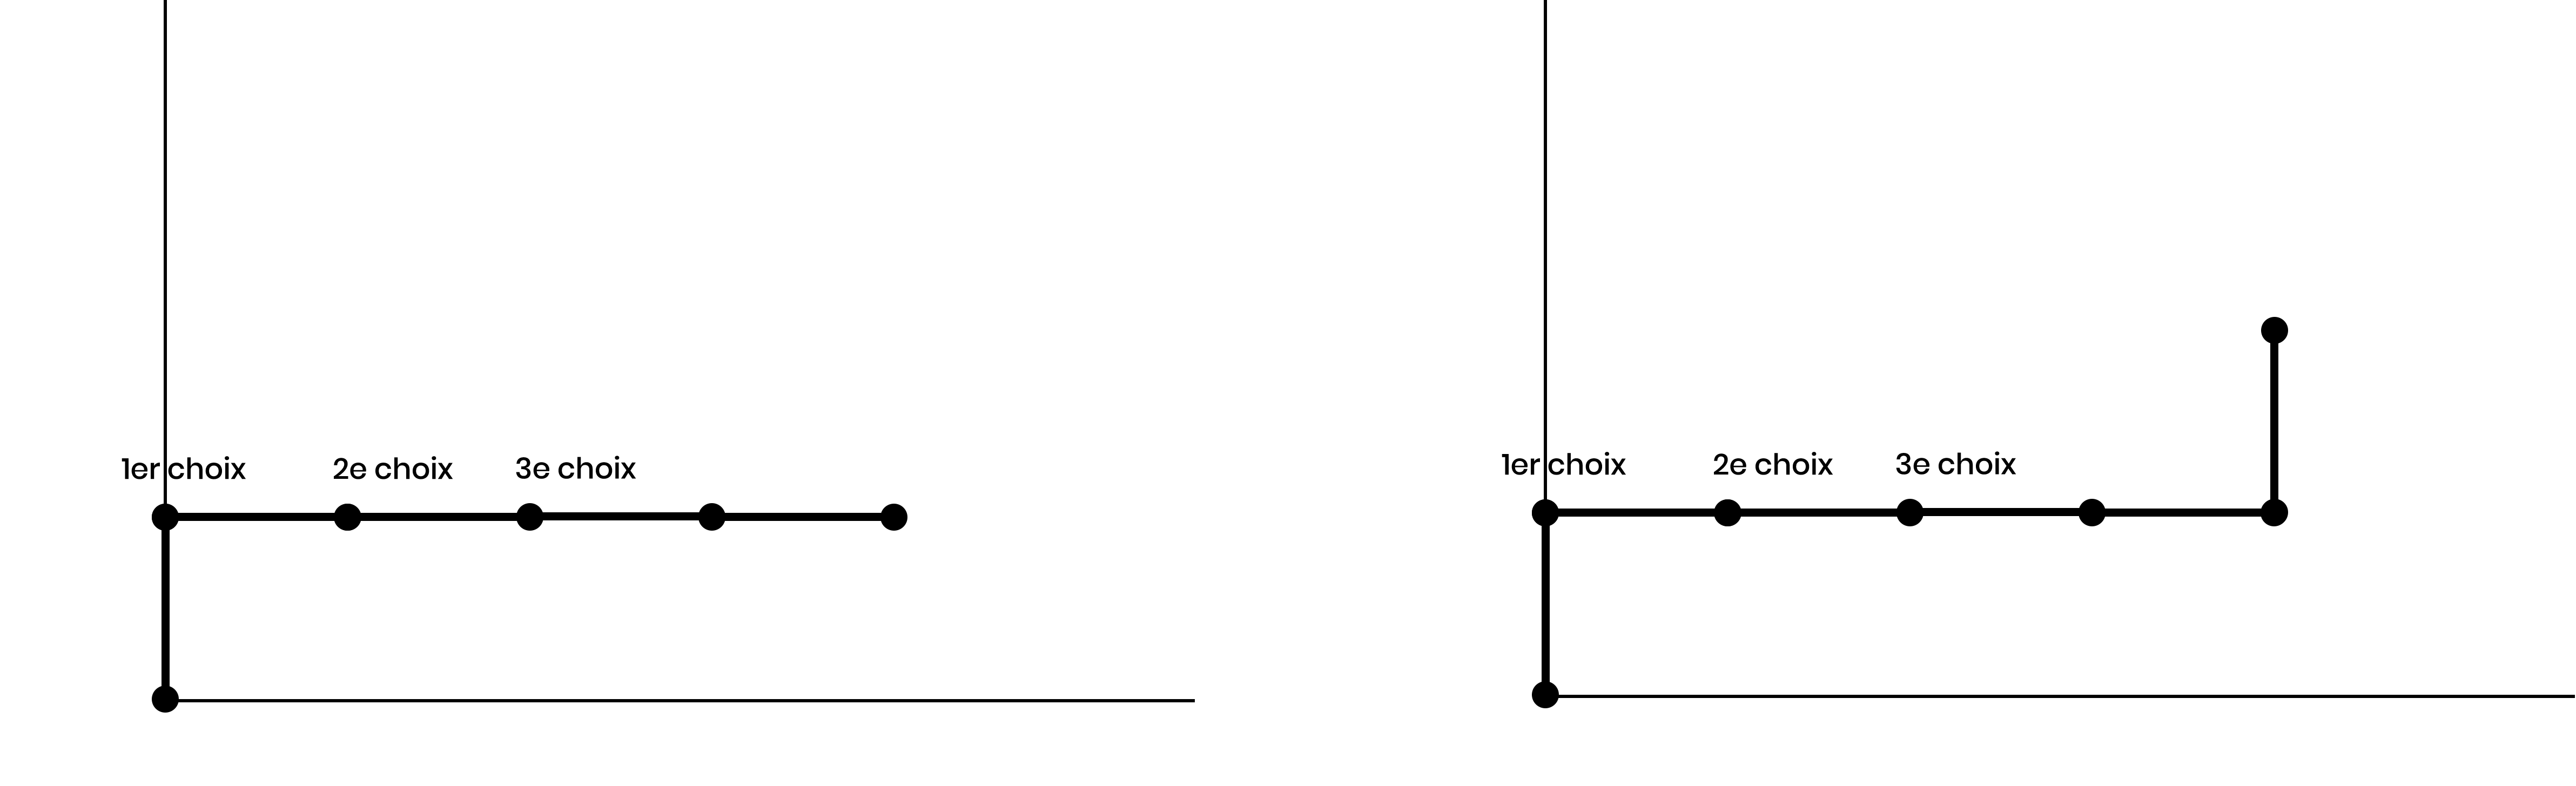
\includegraphics[width=\linewidth]{dedeuxaquatre.png}
\end{figure}

Sur notre exemple, on se place en dimension $2$ (comme dans tout les exemples suivants). On passe du vecteur $(4,1)$ ($(\frac{4}{\sqrt{17}},\frac{1}{\sqrt{17}})$ en normalisé) au vecteur $(4,2)$ ($(\frac{4}{\sqrt{20}},\frac{2}{\sqrt{20}})$ en normalisé). En appliquant la fonction $\mathcal{D}$, on passe de $\frac{5}{\sqrt{20}}$ à $\frac{6}{\sqrt{20}}$. Il y'a donc augmentation de notre fonction $\mathcal{D}$, ce qui traduit bien une augmentation de la diversification. 



\subsection{Méthodes 2 et 3}

Ici, on trouve deux méthodes similaires, et surtout juxtaposables. On modifie légérement notre matrice $\mathcal{M} (U_i)$. On va plutôt considérer un vecteur de taille $N_2 N_1$, noté $X_n$ après la n-ième offre vue, constitué des $N_2$ vecteurs de taille $N_1$ mis bout-à-bout. On travaille ensuite dans l'espace vectoriel $\mathbb{R}^{N_2 N_1}$. Une fois que l'on a accès à ce vecteur, on peut représenter la diversification par des emplacements bien précis dans notre espace vectoriel. \\
On note $e_i$ les vecteurs constitué de $0$ partout et d'un $1$ à la ligne $i$. On considère l'équation d'un hypercone autour de $e_i$, d'angle $\theta$ :

\begin{center}

\[
\displaystyle \sum _{j \neq i} y_j ^2 = y_i ^2 (\tan{\theta}) ^2
\]
\end{center}

On cherche ensuite à garder notre vecteur hors des $N_2 N_1$ cones qui se trouvent autour de chacun des vecteurs unitaires. Pour ce faire, on calcul la quantité :
\end{center}


\begin{center}

\[
\kappa _i = \arctan{\sqrt{\frac{\displaystyle \sum _{j \neq i} <X_n,e_j> ^2}{<X_n,e_i> ^2}}} - \theta
\]

\end{center}

qui nous donne finalement l'angle entre notre vecteur par rapport aux vecteurs générateur de notre cone. On va alors chercher à maximiser chacun de ces angles grâce à nos décisions (ou alors mesurer la diversification en calculant la somme des $\kappa _i$. \\


\begin{figure}[h]
   \caption{Méthode 2 avec des vecteurs non normalisés}
   \includegraphics[width=\linewidth]conerouge.png}
\end{figure}


On peut aussi représenter un hypercone, engendré autour d'une vecteur référence (celui qui possède toutes ses composantes sur la même valeurs). On réalise alors de la même manière un calcul d'angle entre notre vecteur et ce cône, moyennant un changement de base. Finalement, on mesure avec cette méthode l'écart de notre vecteur avec un vecteur référence. Cette méthode se rapproche donc grandement de la méthode numéro une.
 
\begin{figure}[h]
    \caption{Méthode 3 avec des vecteurs non normalisés}
   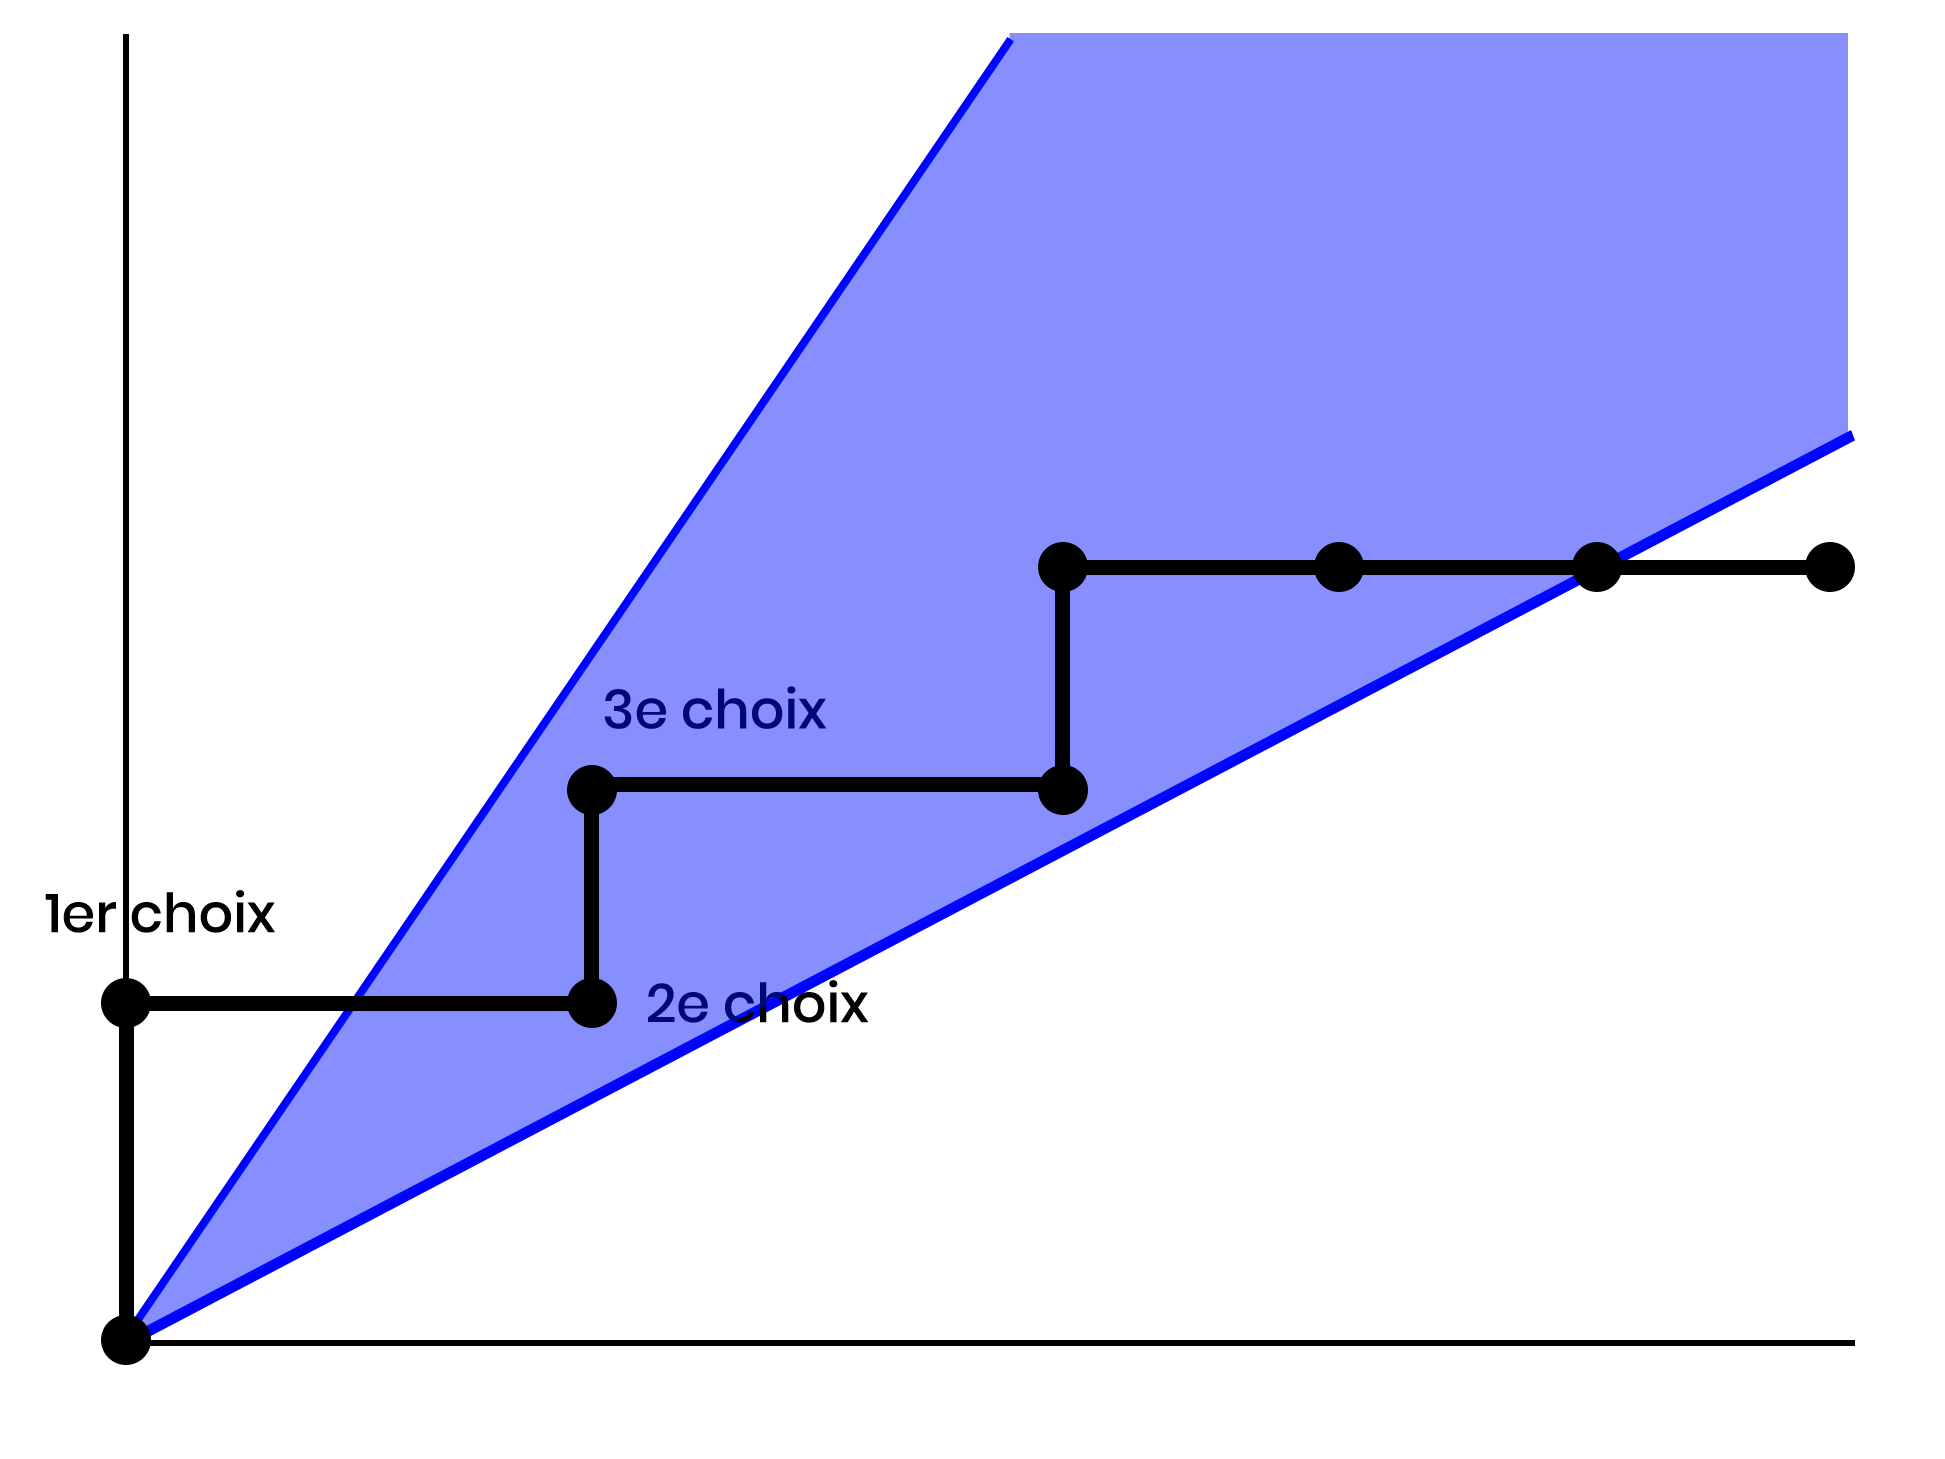
\includegraphics[width=\linewidth]{conebleu.png}
   \caption{Méthodes 2 et 3 avec des vecteurs non normalisés}
   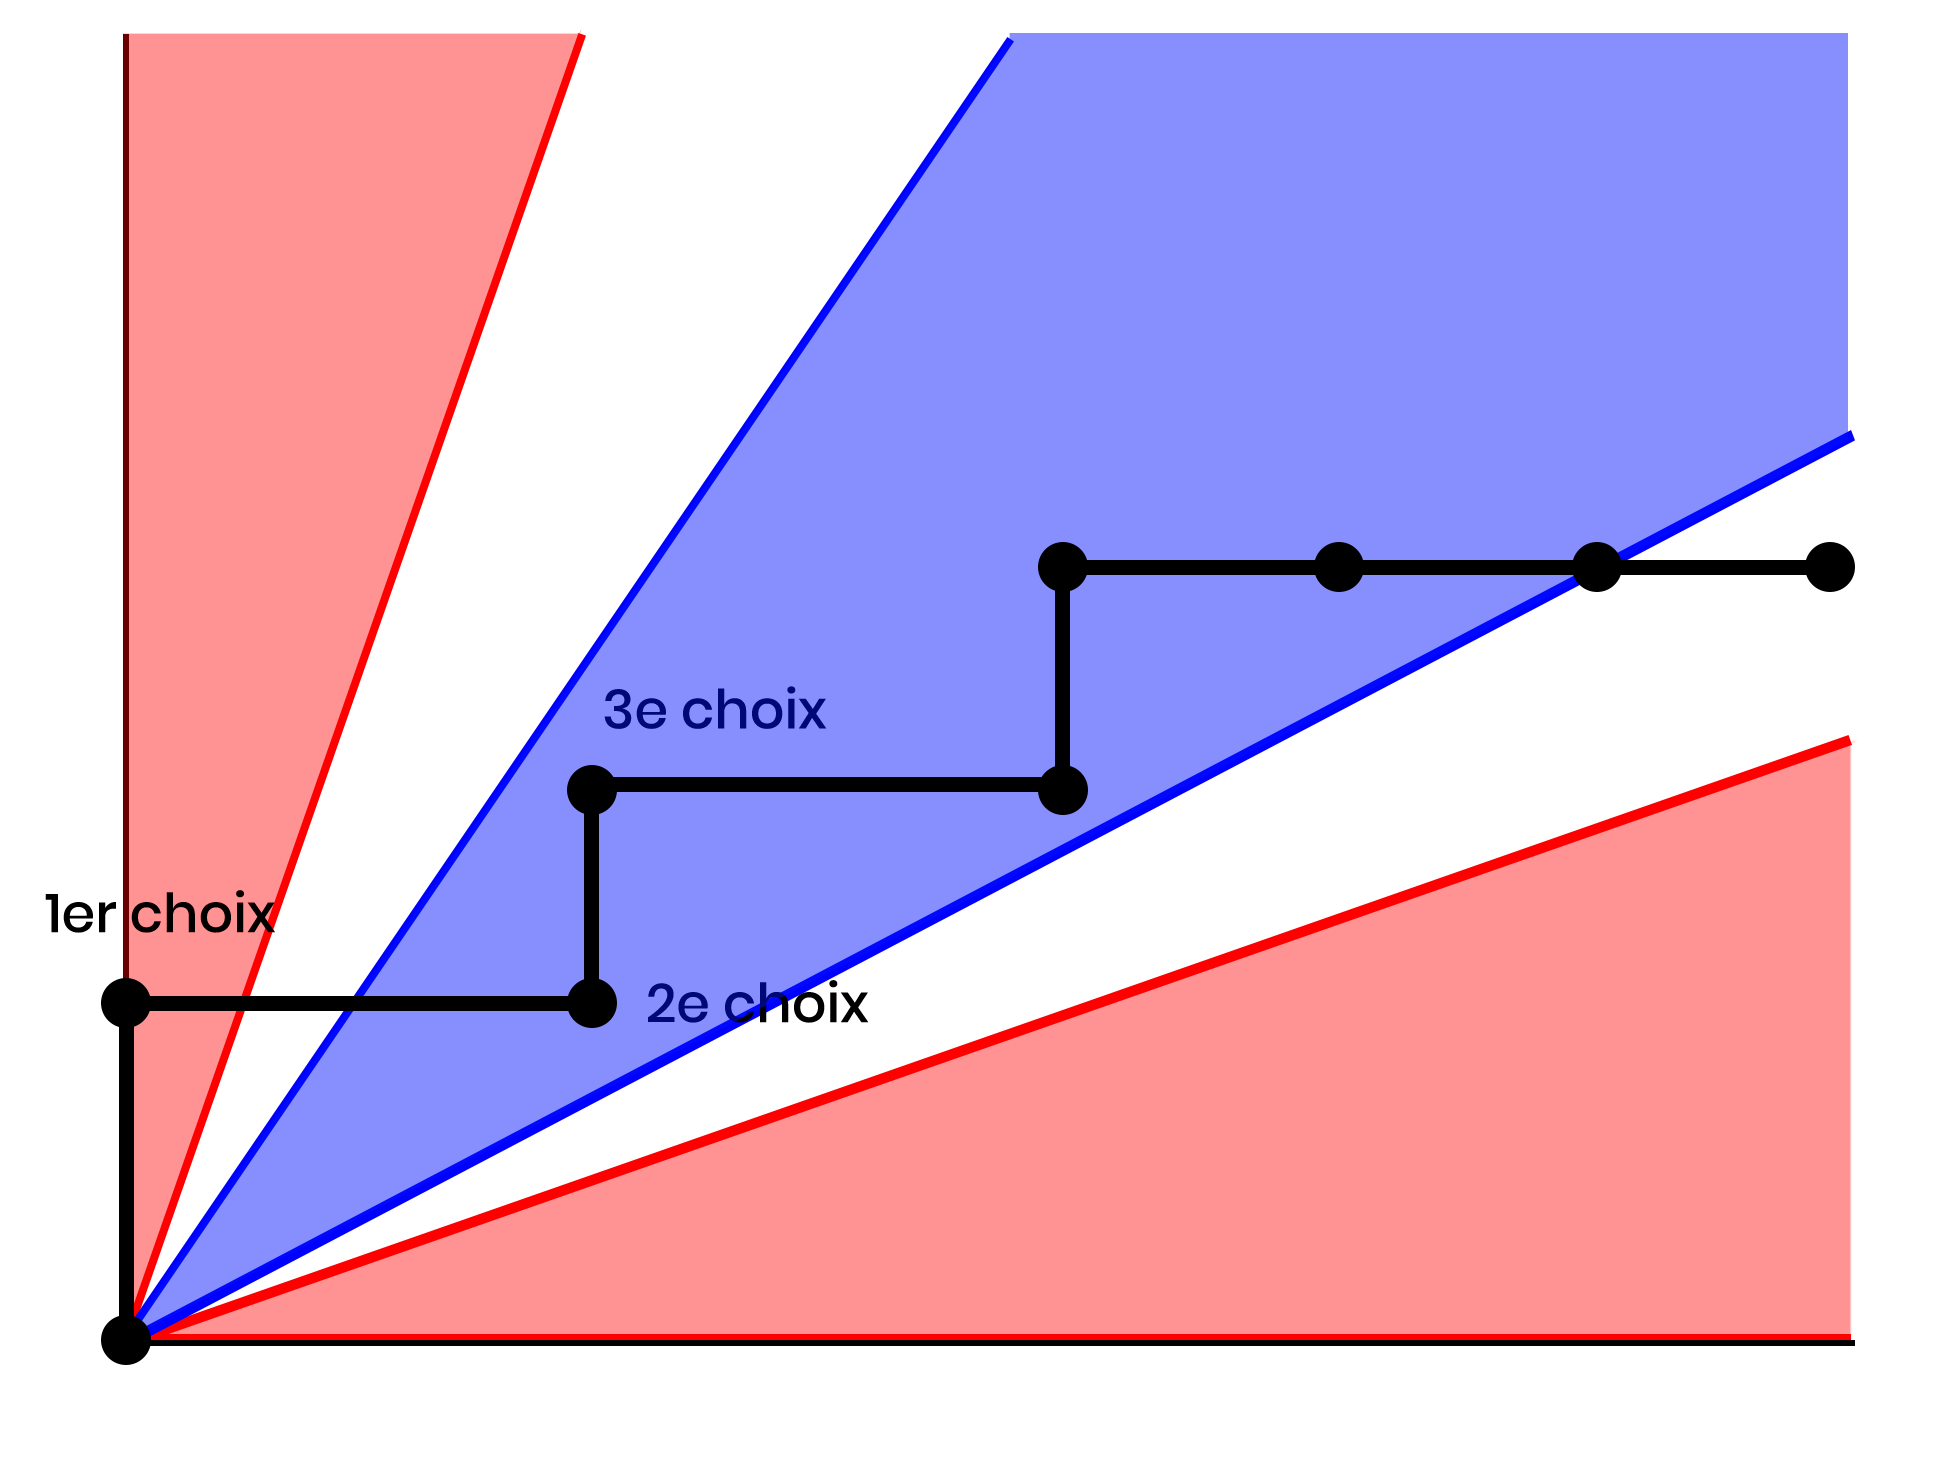
\includegraphics[width=\linewidth]{conerougeetbleu.png}
\end{figure}

\subsection{Méthode 4}

Finalement, une dernière méthode qu'on peut imaginer se justifie de manière assez intuitive. On veut que l'utilisateur sorte de ses habitudes et s'écarte donc de ces dernières. Pour cela, il faut déterminer les habitudes de l'utilisateur.\\
On fixe donc arbitrairement un entier $R\in \mathbb{N}$ représentant le nombre de "choix" d'évènements faits par l'utilisateur qui vont définir son activité récente. Tous les évènements qui datent de $R+1$ choix ou plus seront utilisés pour déterminer les habitudes de l'utilisateur.\\

\begin{figure}[h]
  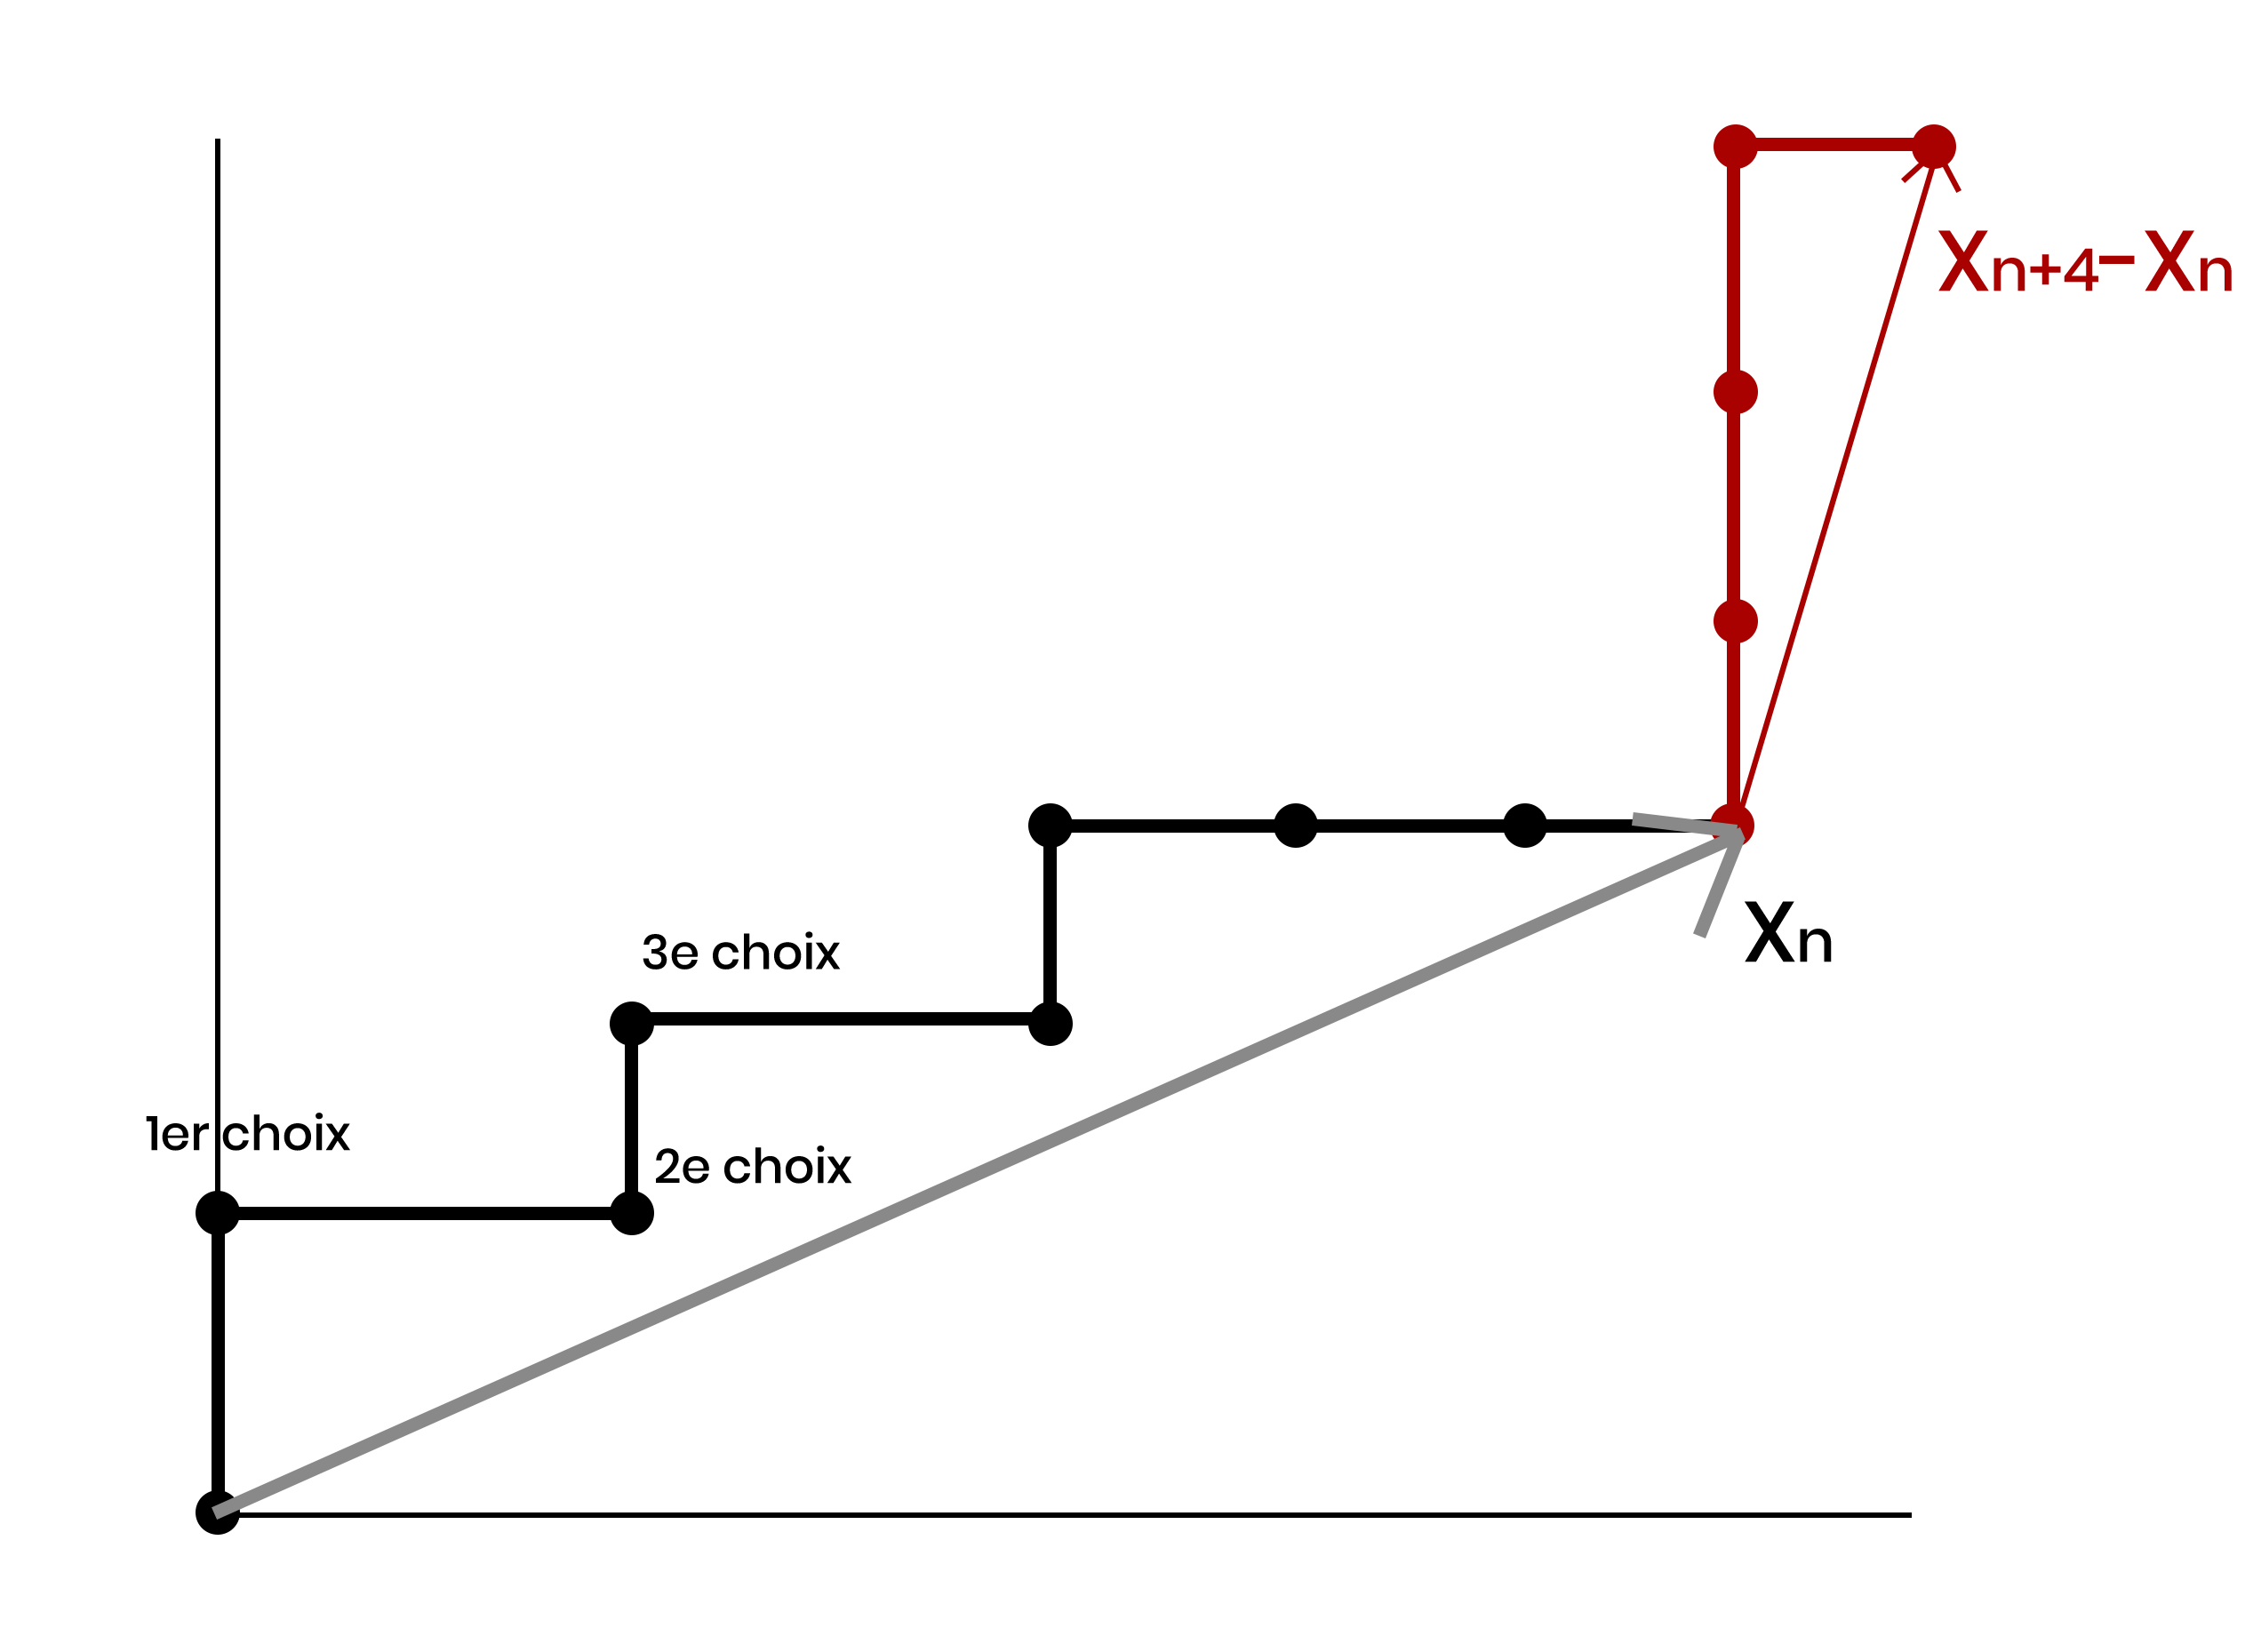
\includegraphics[width=\linewidth]{Visuels/vecteurmoyen.png}
  \caption{Méthode 4 - Représentation de l'habitude de l'utilisateur pour R=4}
  \label{fig:methodequatre}
\end{figure}

On peut voir sur la \ref{fig:methodequatre}, dans un cadre à deux dimensions avec $R=4$, l'habitude de l'utilisateur représentée par le vecteur $X_{n}$ en noir, et son activité récente représentée par le vecteur $X_{n+4}-X_{n}$ en rouge.\\
L'idée est donc de faire en sorte que chaque activité récente s'écarte des habitudes de l'utilisateur. Par conséquent, on va chercher à minimiser la quantité:
$$|<X_{n},X_{n+4}-X_{n}>|=|<X_{n},X_{n+4}>-||X_{n}||^{2}|=|<X_{n},X_{n+4}>-1|$$
Ce qui revient simplement

\section{En pratique}

Une fois la mesure de diversification d'un utilisateur réalisée, il faut regarder comment la faire évoluer. De par sa définition, il nous semble qu'on ne peut se baser sur les caractéristiques de l'utilisateur en lui même pour choisir un événement (justement car on veut le faire changer, et qu'en plus, il faut que ce nouveau type d'événement puisse lui plaire). On va donc combiner deux autres méthodes : une se basant sur les événements se rapprochant de ce qu'il aime, et une se basant sur les utilisateurs qui lui ressemblent. \\

On va commencer par classer les composants de la matrice $\mathcal{M} (U_i)$ par ordre croissant. Ensuite, on va extraire les composants qui nous intéressent (par exemple les 5 moins bons, ou alors les 10 autour de la moyenne). Chacun de ces composants sont liés à un type d'événement bien défini. \\

En parallèle, on réalise un double classement (grâce aux méthodes vu précédemment dans les autres sections) des événements qui satisfairont le plus l'utilisateur d'après les gens et les événements qui lui ressemblent. \\

On extrait alors de ce classement un nouveau classement qui ne comprend que les types d'événements liés aux composants selectionnés. On classe une seconde fois les événements choisis grâce au calcul de la diversification qu'ils entraîneraient sur l'utilisateur. Ensuite, on réalise un classement en prenant en compte les deux classements précédents, et on envoie les offres à l'utilisateur.  \\ 



\end{document}